\documentclass[aspectratio=169,11pt]{beamer}

% Theme and colors
\usetheme{Madrid}
\usecolortheme{whale}
\setbeamertemplate{navigation symbols}{}
\setbeamertemplate{footline}[frame number]

% Packages
\usepackage[utf8]{inputenc}
\usepackage[T1]{fontenc}
\usepackage{graphicx}
\usepackage{booktabs}
\usepackage{amsmath}
\usepackage{hyperref}
\usepackage{tikz}
\usetikzlibrary{shapes,arrows,positioning,calc,fit,backgrounds}
\usepackage{xcolor}
\usepackage{array}
\usepackage{listings}
\usepackage{fontawesome5}

% Listing style for code
\lstset{
    basicstyle=\ttfamily\scriptsize,
    breaklines=true,
    frame=single,
    backgroundcolor=\color{gray!10},
    keywordstyle=\color{blue!70},
    commentstyle=\color{green!50!black},
    stringstyle=\color{red!60},
    showstringspaces=false,
    tabsize=2
}

% Custom colors
\definecolor{stepbg}{RGB}{232,245,233}
\definecolor{stepborder}{RGB}{76,175,80}
\definecolor{aibg}{RGB}{243,229,245}
\definecolor{aiborder}{RGB}{156,39,176}
\definecolor{verifybg}{RGB}{227,242,253}
\definecolor{verifyborder}{RGB}{33,150,243}
\definecolor{hwbg}{RGB}{255,243,224}
\definecolor{hwborder}{RGB}{255,152,0}
\definecolor{tryitbg}{RGB}{255,253,231}
\definecolor{tryitborder}{RGB}{198,167,0}

% Title information
\title[EECE5155 -- Cloud IoT Seminar]{Cloud IoT Pipeline: Hands-On Seminar}
\subtitle{MQTT $\rightarrow$ InfluxDB $\rightarrow$ Grafana in 60 Minutes}
\author{Eduardo Baena}
\date{Thursday, March 20, 2026}
\institute{Northeastern University\\Department of Electrical and Computer Engineering\\
\texttt{e.baena@northeastern.edu}}

\begin{document}

% Title slide
\begin{frame}
    \titlepage
    \vspace{-0.8cm}
    \begin{center}
        \textbf{EECE5155: Wireless Sensor Networks and the Internet of Things}\\[4pt]
        {\small Everything runs on \textbf{your laptop}. No cloud account needed.}
    \end{center}
\end{frame}

%==============================================================================
\section{Overview}
%==============================================================================

\begin{frame}{What We Are Building Today}
    \begin{center}
    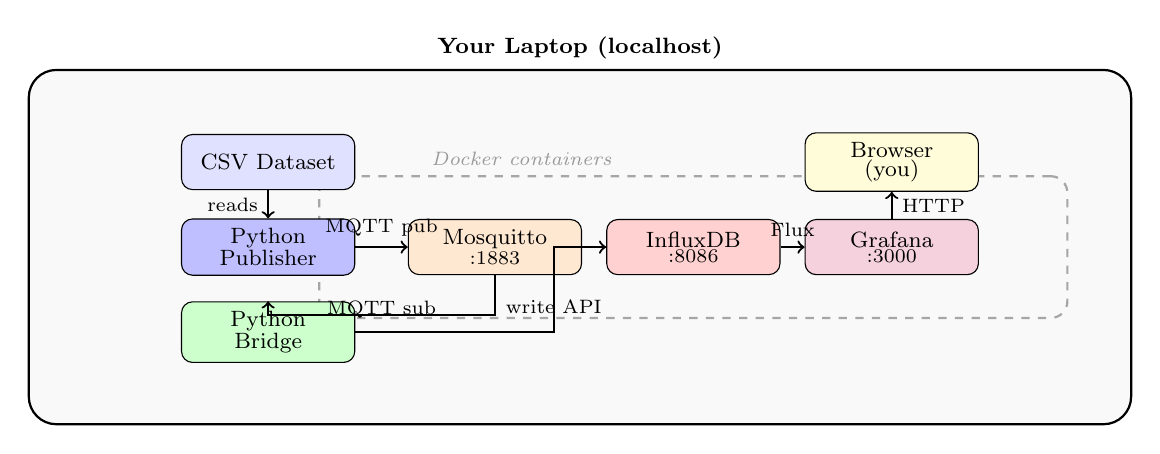
\begin{tikzpicture}[
        scale=0.72,
        every node/.style={font=\footnotesize},
        box/.style={draw, minimum width=2.2cm, minimum height=0.7cm, rounded corners},
        docker/.style={draw, dashed, thick, gray!70, rounded corners=6pt},
    ]
        % --- Laptop boundary ---
        \node[draw, thick, rounded corners=10pt, minimum width=14cm, minimum height=4.5cm,
              fill=gray!5, label={[font=\footnotesize\bfseries]above:Your Laptop (localhost)}] at (6,-1.5) {};

        % --- Docker boundary ---
        \node[docker, minimum width=9.5cm, minimum height=1.8cm,
              label={[font=\scriptsize\itshape, gray!80]above left:Docker containers}] at (8,-1.5) {};

        % --- Python scripts (outside Docker) ---
        \node[box, fill=blue!12]  (csv)    at (0.5, 0)    {CSV Dataset};
        \node[box, fill=blue!25]  (pub)    at (0.5,-1.5)  {\shortstack{Python\\[-2pt]Publisher}};
        \node[box, fill=green!20] (bridge) at (0.5,-3)    {\shortstack{Python\\[-2pt]Bridge}};

        % --- Docker services ---
        \node[box, fill=orange!18] (mqtt)    at (4.5,-1.5) {\shortstack{Mosquitto\\[-2pt]\scriptsize :1883}};
        \node[box, fill=red!18]    (influx)  at (8,-1.5)   {\shortstack{InfluxDB\\[-2pt]\scriptsize :8086}};
        \node[box, fill=purple!18] (grafana) at (11.5,-1.5) {\shortstack{Grafana\\[-2pt]\scriptsize :3000}};

        % --- Browser ---
        \node[box, fill=yellow!15] (browser) at (11.5, 0)  {\shortstack{Browser\\[-2pt](you)}};

        % --- Arrows ---
        \draw[->, thick] (csv) -- node[left, font=\scriptsize]{reads} (pub);
        \draw[->, thick] (pub) -- node[above, font=\scriptsize]{MQTT pub} (mqtt);
        \draw[->, thick] (mqtt.south) -- ++(0,-0.7) -| (bridge.north);
        \node[font=\scriptsize] at (2.5,-2.6) {MQTT sub};
        \draw[->, thick] (bridge.east) -- ++(3.5,0) |- node[below, font=\scriptsize, pos=0.25]{write API} (influx);
        \draw[->, thick] (influx) -- node[above, font=\scriptsize]{Flux} (grafana);
        \draw[->, thick] (grafana) -- node[right, font=\scriptsize]{HTTP} (browser);
    \end{tikzpicture}
    \end{center}

    \vspace{-0.1cm}
    \begin{columns}
        \column{0.48\textwidth}
        \textbf{You write (Python):}
        \begin{itemize}
            \item \texttt{mqtt\_publisher.py} --- CSV $\rightarrow$ MQTT
            \item \texttt{mqtt\_bridge.py} --- MQTT $\rightarrow$ InfluxDB
        \end{itemize}

        \column{0.48\textwidth}
        \textbf{Docker runs for you:}
        \begin{itemize}
            \item Mosquitto broker (\texttt{:1883})
            \item InfluxDB time-series DB (\texttt{:8086})
            \item Grafana dashboards (\texttt{:3000})
        \end{itemize}
    \end{columns}
\end{frame}

\begin{frame}{Seminar Rules}
    \begin{columns}
        \column{0.55\textwidth}
        \textbf{Today (in-class, 60 min):}
        \begin{enumerate}
            \item Follow the slides step by step
            \item Type the commands yourself
            \item If you get stuck, ask me or a neighbor
            \item \textbf{Goal:} see data flow from CSV to Grafana
        \end{enumerate}

        \vspace{0.3cm}
        \textbf{AI policy:}
        \begin{itemize}
            \item \textbf{Today:} follow the slides, don't use AI yet
            \item \textbf{Take-home tasks:} AI is encouraged
            \item Always \textbf{verify} AI output by running the code
        \end{itemize}

        \column{0.42\textwidth}
        \begin{exampleblock}{Grading}
            Working code with no explanation: \textbf{50\%}\\[4pt]
            Broken code with debugging log: \textbf{80\%}\\[4pt]
            Working code + reasoning + AI audit: \textbf{100\%}
        \end{exampleblock}

        \vspace{0.2cm}
        \begin{alertblock}{Timeline}
            \textbf{0--20 min:} MQTT\\
            \textbf{20--40 min:} InfluxDB bridge\\
            \textbf{40--60 min:} Grafana dashboard\\[4pt]
            \textbf{Take-home:} 3 AI tasks (due next Wed)
        \end{alertblock}
    \end{columns}
\end{frame}

%==============================================================================
\section{Step 0: Setup (do this BEFORE class)}
%==============================================================================

\begin{frame}[fragile]{Step 0a: Install Tools --- Before Class}
    \fcolorbox{stepborder}{stepbg}{\begin{minipage}{0.93\textwidth}
    \textbf{\faIcon{check-circle} Complete these steps \underline{before} the seminar.}
    \end{minipage}}

    \vspace{0.2cm}
    \textbf{1. Docker Desktop} --- download from \texttt{docker.com}, make sure it is running

    \vspace{0.1cm}
    \textbf{2. Clone the seminar repo:}
\begin{lstlisting}[language=bash]
git clone https://github.com/ebaenamar/ECE5155_practical_iot_cloud.git
cd ECE5155_practical_iot_cloud
\end{lstlisting}

    \vspace{0.1cm}
    \textbf{3. Python dependencies:}
\begin{lstlisting}[language=bash]
python3 -m venv .venv && source .venv/bin/activate
pip install -r requirements.txt
\end{lstlisting}

    \vspace{0.1cm}
    \textbf{4. Start the infrastructure:}
\begin{lstlisting}[language=bash]
docker compose up -d
\end{lstlisting}
\end{frame}

\begin{frame}[fragile]{Step 0b: Download the Dataset from Kaggle}
    \fcolorbox{stepborder}{stepbg}{\begin{minipage}{0.93\textwidth}
    \textbf{\faIcon{database} You need a free Kaggle account to download the CSV.}
    \end{minipage}}

    \vspace{0.2cm}
    \textbf{Create a Kaggle account} (if you don't have one):
    \begin{enumerate}
        \item Go to \texttt{kaggle.com} $\rightarrow$ \textbf{Register} (or sign in with Google)
    \end{enumerate}

    \vspace{0.1cm}
    \textbf{Download the dataset:}
    \begin{enumerate}
        \item Go to: {\footnotesize\texttt{kaggle.com/datasets/atulanandjha/temperature-readings-iot-devices}}
        \item Click \textbf{Download} (top right) $\rightarrow$ unzip the file
        \item Move \texttt{IOT-temp.csv} into the \texttt{ECE5155\_practical\_iot\_cloud/} folder
    \end{enumerate}

    \vspace{0.1cm}
    \textbf{Verify everything works:}
\begin{lstlisting}[language=bash]
docker compose ps               # 3 services running
curl localhost:8086/health       # {"status":"pass"}
curl localhost:3000/api/health   # {"status":"ok"}
head -2 IOT-temp.csv            # id,room_id/id,noted_date,temp,out/in
\end{lstlisting}

    \vspace{0.1cm}
    \fcolorbox{verifyborder}{verifybg}{\begin{minipage}{0.93\textwidth}
    \textbf{\faIcon{check} If all 4 checks pass, you are ready for the seminar!}
    \end{minipage}}
\end{frame}

%==============================================================================
\section{Part 1: MQTT (0--20 min)}
%==============================================================================

\begin{frame}[fragile]{Part 1: MQTT --- What You Need to Know}
    \begin{columns}
        \column{0.55\textwidth}
        \textbf{MQTT in 30 seconds:}
        \begin{itemize}
            \item Publish/subscribe messaging protocol
            \item Devices publish to \textbf{topics} (strings)
            \item Clients subscribe with \textbf{wildcards}
            \item A \textbf{broker} (Mosquitto) routes messages
            \item Lightweight --- designed for IoT
        \end{itemize}

        \vspace{0.2cm}
        \textbf{Our topic design:}\\
        \texttt{iot/\{room\}/\{In|Out\}/temp}

        \vspace{0.1cm}
        Examples:
        \begin{itemize}
            \item \texttt{iot/Room Admin/In/temp}
            \item \texttt{iot/Room Admin/Out/temp}
        \end{itemize}

        \column{0.42\textwidth}
        \textbf{Wildcards:}
        \begin{itemize}
            \item \texttt{iot/\#} --- all IoT messages
            \item \texttt{iot/+/In/temp} --- all indoor
            \item \texttt{iot/+/Out/temp} --- all outdoor
        \end{itemize}

        \vspace{0.2cm}
        \textbf{Payload:} JSON
\begin{lstlisting}
{
  "device_id": "log_196134",
  "temp": 29.0,
  "ts": "08-12-2018 09:30"
}
\end{lstlisting}
    \end{columns}
\end{frame}

\begin{frame}[fragile]{Step 1: Test MQTT with the Command Line}
    \fcolorbox{stepborder}{stepbg}{\begin{minipage}{0.93\textwidth}
    \textbf{\faIcon{terminal} Open two terminals side by side.}
    \end{minipage}}

    \vspace{0.3cm}
    \textbf{Terminal 1 --- Subscribe (listener):}
\begin{lstlisting}[language=bash]
docker exec -it seminar_test-mosquitto-1 \
    mosquitto_sub -t "iot/#" -v
\end{lstlisting}
    {\small This will wait and print any message that arrives on \texttt{iot/\#}.}

    \vspace{0.3cm}
    \textbf{Terminal 2 --- Publish (sender):}
\begin{lstlisting}[language=bash]
docker exec -it seminar_test-mosquitto-1 \
    mosquitto_pub -t "iot/Room Admin/In/temp" \
    -m '{"device_id":"test","temp":25.3,"ts":"now"}'
\end{lstlisting}

    \vspace{0.2cm}
    \fcolorbox{verifyborder}{verifybg}{\begin{minipage}{0.93\textwidth}
    \textbf{\faIcon{check} Verify:} You should see the message appear in Terminal 1 immediately.
    \end{minipage}}
\end{frame}

\begin{frame}[fragile]{\faIcon{flask} Try It: Explore MQTT Topics \& Wildcards}
    \fcolorbox{tryitborder}{tryitbg}{\begin{minipage}{0.93\textwidth}
    \textbf{\faIcon{hand-point-right} Do these experiments before moving on. Discuss with your neighbor.}
    \end{minipage}}

    \vspace{0.2cm}
    \textbf{Experiment 1:} Publish to a \textbf{different topic}. In Terminal 2:
\begin{lstlisting}[language=bash]
mosquitto_pub -t "iot/Kitchen/In/temp" \
    -m '{"device_id":"k1","temp":22.5,"ts":"now"}'
\end{lstlisting}
    {\small $\rightarrow$ Does it appear in Terminal 1? \textbf{Why?} (hint: \texttt{iot/\#})}

    \vspace{0.15cm}
    \textbf{Experiment 2:} Stop the subscriber (Ctrl+C). Restart with a \textbf{specific wildcard}:
\begin{lstlisting}[language=bash]
mosquitto_sub -t "iot/+/Out/temp" -v
\end{lstlisting}
    Now publish one \texttt{In} message and one \texttt{Out} message. Which one appears?

    \vspace{0.15cm}
    \textbf{Experiment 3:} Publish a message with a \textbf{bad JSON} payload:
\begin{lstlisting}[language=bash]
mosquitto_pub -t "iot/Lab/In/temp" -m "not json at all"
\end{lstlisting}
    {\small $\rightarrow$ What happens? MQTT doesn't care about the payload format --- the broker just routes bytes.}
\end{frame}

\begin{frame}[fragile]{Step 2: Write the Python Publisher}
    \fcolorbox{stepborder}{stepbg}{\begin{minipage}{0.93\textwidth}
    \textbf{\faIcon{python} Create \texttt{mqtt\_publisher.py} --- reads the CSV and publishes each row.}
    \end{minipage}}

    \vspace{0.05cm}
\begin{lstlisting}[language=Python]
import paho.mqtt.client as mqtt
import csv, json, time

client = mqtt.Client(mqtt.CallbackAPIVersion.VERSION2)
client.connect("localhost", 1883, 60)

with open("IOT-temp.csv") as f:
    reader = csv.DictReader(f)
    count = 0
    for row in reader:
        room = row.get("room_id/id", "unknown").strip()
        loc  = row.get("out/in", "unknown").strip()
        topic = f"iot/{room}/{loc}/temp"
        payload = json.dumps({
            "device_id": row["id"].strip(),
            "temp": float(row["temp"]),
            "ts": row["noted_date"].strip()
        })
        client.publish(topic, payload, qos=1)
        count += 1
        if count % 1000 == 0:
            print(f"Sent {count} messages")
        time.sleep(0.01)   # ~100 msg/sec
\end{lstlisting}
\end{frame}

\begin{frame}[fragile]{Step 3: Run Publisher + Verify}
    \fcolorbox{stepborder}{stepbg}{\begin{minipage}{0.93\textwidth}
    \textbf{\faIcon{play} Run the publisher. Keep Terminal 1 (subscriber) open.}
    \end{minipage}}

    \vspace{0.3cm}
    \textbf{Terminal 2:}
\begin{lstlisting}[language=bash]
python mqtt_publisher.py
\end{lstlisting}

    \vspace{0.2cm}
    You should see:
\begin{lstlisting}
Sent 1000 messages
Sent 2000 messages
...
\end{lstlisting}

    And in Terminal 1 (the \texttt{mosquitto\_sub} window), messages scrolling:
\begin{lstlisting}
iot/Room Admin/In/temp {"device_id":"...", "temp":29.0, ...}
iot/Room Admin/Out/temp {"device_id":"...", "temp":36.0, ...}
\end{lstlisting}

    \vspace{0.2cm}
    \fcolorbox{verifyborder}{verifybg}{\begin{minipage}{0.93\textwidth}
    \textbf{\faIcon{check} Checkpoint:} Stop the publisher after $\sim$3000 messages (Ctrl+C).\\
    You now have working MQTT publish/subscribe. \textbf{Part 1 done.}
    \end{minipage}}
\end{frame}

\begin{frame}[fragile]{\faIcon{flask} Try It: Inspect the Publisher Output}
    \fcolorbox{tryitborder}{tryitbg}{\begin{minipage}{0.93\textwidth}
    \textbf{\faIcon{hand-point-right} Answer these questions by observing the subscriber output.}
    \end{minipage}}

    \vspace{0.2cm}
    \textbf{Question 1:} How many \textbf{unique topics} do you see? List them.\\
    {\small (Hint: look at the left side of each line in \texttt{mosquitto\_sub})}

    \vspace{0.2cm}
    \textbf{Question 2:} Are indoor temperatures generally higher or lower than outdoor?\\
    {\small Pick 3 consecutive \texttt{In} and 3 \texttt{Out} messages --- compare the \texttt{temp} values.}

    \vspace{0.2cm}
    \textbf{Question 3:} Modify the publisher code to also publish a \textbf{second field}.\\
    Add \texttt{"room": room} to the JSON payload. Re-run and verify it shows in the subscriber.

    \vspace{0.2cm}
    \textbf{Question 4:} What happens if you change \texttt{qos=1} to \texttt{qos=0} in the publisher?\\
    {\small Run both versions. Can you notice any difference in speed or message delivery?}

    \vspace{0.1cm}
    \fcolorbox{verifyborder}{verifybg}{\begin{minipage}{0.93\textwidth}
    \textbf{\faIcon{users} Discuss:} Why might QoS 1 matter for a real sensor deployment but not for this CSV replay?
    \end{minipage}}
\end{frame}

%==============================================================================
\section{Part 2: MQTT $\rightarrow$ InfluxDB (20--40 min)}
%==============================================================================

\begin{frame}{Part 2: InfluxDB --- What You Need to Know}
    \begin{columns}
        \column{0.52\textwidth}
        \textbf{InfluxDB in 30 seconds:}
        \begin{itemize}
            \item Time-series database (optimized for IoT)
            \item Data model:
            \begin{itemize}
                \item \textbf{Measurement:} like a table name
                \item \textbf{Tags:} indexed metadata (room, location)
                \item \textbf{Fields:} the actual values (temperature)
                \item \textbf{Timestamp:} when it happened
            \end{itemize}
            \item Query language: \textbf{Flux}
        \end{itemize}

        \column{0.45\textwidth}
        \textbf{Our data model:}

        \vspace{0.1cm}
        \footnotesize
        \begin{tabular}{ll}
            \toprule
            \textbf{Concept} & \textbf{Value} \\
            \midrule
            Bucket & \texttt{iot-sensors} \\
            Measurement & \texttt{temperature} \\
            Tag: room\_id & \texttt{Room Admin} \\
            Tag: location & \texttt{In} or \texttt{Out} \\
            Field: value & \texttt{29.0} \\
            Timestamp & from CSV \\
            \bottomrule
        \end{tabular}
        \normalsize

        \vspace{0.2cm}
        \textbf{Already configured:}\\
        {\small Org: \texttt{eece5155}\\
        Bucket: \texttt{iot-sensors}\\
        Token: \texttt{seminar-test-token}}
    \end{columns}
\end{frame}

\begin{frame}[fragile]{Step 4: Write the MQTT-to-InfluxDB Bridge}
    \fcolorbox{stepborder}{stepbg}{\begin{minipage}{0.93\textwidth}
    \textbf{\faIcon{python} Create \texttt{mqtt\_bridge.py} --- subscribes to MQTT, writes to InfluxDB.}
    \end{minipage}}

    \vspace{-0.05cm}
\begin{lstlisting}[language=Python,basicstyle=\ttfamily\tiny]
from influxdb_client import InfluxDBClient, Point
from influxdb_client.client.write_api import SYNCHRONOUS
import paho.mqtt.client as mqtt, json

influx = InfluxDBClient(url="http://localhost:8086",
                        token="seminar-test-token", org="eece5155")
write_api = influx.write_api(write_options=SYNCHRONOUS)
count = 0

def on_message(client, userdata, msg):
    global count
    data = json.loads(msg.payload)
    parts = msg.topic.split("/")
    point = (Point("temperature")
        .tag("room_id", parts[1] if len(parts) > 1 else "unknown")
        .tag("location", parts[2] if len(parts) > 2 else "unknown")
        .field("value", data["temp"]))
    write_api.write(bucket="iot-sensors", record=point)
    count += 1
    if count % 500 == 0:
        print(f"Written {count} points to InfluxDB")

mqtt_client = mqtt.Client(mqtt.CallbackAPIVersion.VERSION2)
mqtt_client.on_message = on_message
mqtt_client.connect("localhost", 1883)
mqtt_client.subscribe("iot/#")
print("Bridge running... waiting for MQTT messages")
mqtt_client.loop_forever()
\end{lstlisting}
\end{frame}

\begin{frame}[fragile]{Step 5: Run the Bridge + Publisher Together}
    \fcolorbox{stepborder}{stepbg}{\begin{minipage}{0.93\textwidth}
    \textbf{\faIcon{play} Two terminals. Bridge first, then publisher.}
    \end{minipage}}

    \vspace{0.3cm}
    \textbf{Terminal 1 --- Bridge:}
\begin{lstlisting}[language=bash]
python mqtt_bridge.py
\end{lstlisting}
    {\small Output: \texttt{Bridge running... waiting for MQTT messages}}

    \vspace{0.2cm}
    \textbf{Terminal 2 --- Publisher:}
\begin{lstlisting}[language=bash]
python mqtt_publisher.py
\end{lstlisting}

    \vspace{0.2cm}
    Terminal 1 will show:
\begin{lstlisting}
Written 500 points to InfluxDB
Written 1000 points to InfluxDB
Written 1500 points to InfluxDB
...
\end{lstlisting}

    \vspace{0.1cm}
    {\small Let it run for $\sim$2 minutes ($\sim$10,000+ points), then Ctrl+C both.}

    \vspace{0.1cm}
    \fcolorbox{verifyborder}{verifybg}{\begin{minipage}{0.93\textwidth}
    \textbf{\faIcon{check} Checkpoint:} Data is now flowing: CSV $\rightarrow$ MQTT $\rightarrow$ InfluxDB. \textbf{Part 2 almost done.}
    \end{minipage}}
\end{frame}

\begin{frame}[fragile]{Step 6: Verify Data in InfluxDB}
    \fcolorbox{stepborder}{stepbg}{\begin{minipage}{0.93\textwidth}
    \textbf{\faIcon{globe} Open your browser: \texttt{http://localhost:8086}}\\
    {\small Login: \texttt{admin} / \texttt{admin12345}}
    \end{minipage}}

    \vspace{0.3cm}
    \textbf{In the InfluxDB UI:}
    \begin{enumerate}
        \item Click \textbf{Data Explorer} (left sidebar)
        \item Select bucket: \texttt{iot-sensors}
        \item Select measurement: \texttt{temperature}
        \item Click \textbf{Submit} --- you should see data points
    \end{enumerate}

    \vspace{0.2cm}
    \textbf{Try this Flux query} (click ``Script Editor''):
\begin{lstlisting}
from(bucket: "iot-sensors")
  |> range(start: -30d)
  |> filter(fn: (r) => r._measurement == "temperature")
  |> filter(fn: (r) => r._field == "value")
  |> group(columns: ["location"])
  |> mean()
\end{lstlisting}

    \vspace{0.1cm}
    \fcolorbox{verifyborder}{verifybg}{\begin{minipage}{0.93\textwidth}
    \textbf{\faIcon{check} Checkpoint:} You see average temperature for In vs Out. \textbf{Part 2 done.}
    \end{minipage}}
\end{frame}

\begin{frame}[fragile]{\faIcon{flask} Try It: Explore InfluxDB Queries}
    \fcolorbox{tryitborder}{tryitbg}{\begin{minipage}{0.93\textwidth}
    \textbf{\faIcon{hand-point-right} Write these Flux queries in the InfluxDB Data Explorer. Observe the results.}
    \end{minipage}}

    \vspace{0.15cm}
    \textbf{Query 1:} How many data points did you ingest \textbf{in total}?
\begin{lstlisting}
from(bucket: "iot-sensors")
  |> range(start: -30d)
  |> filter(fn: (r) => r._measurement == "temperature")
  |> count()
\end{lstlisting}

    \vspace{0.1cm}
    \textbf{Query 2:} What is the \textbf{max temperature} per room?
\begin{lstlisting}
from(bucket: "iot-sensors")
  |> range(start: -30d)
  |> filter(fn: (r) => r._measurement == "temperature")
  |> filter(fn: (r) => r._field == "value")
  |> group(columns: ["room_id"])
  |> max()
\end{lstlisting}

    \vspace{0.1cm}
    \textbf{Question:} Which room has the highest temperature? Is it indoor or outdoor?
\end{frame}

%==============================================================================
\section{Part 3: Grafana Dashboard (40--60 min)}
%==============================================================================

\begin{frame}[fragile]{Step 7: Open Grafana and Check the Data Source}
    \fcolorbox{stepborder}{stepbg}{\begin{minipage}{0.93\textwidth}
    \textbf{\faIcon{globe} Open: \texttt{http://localhost:3000}}\\
    {\small Login: \texttt{admin} / \texttt{admin} (skip password change)}
    \end{minipage}}

    \vspace{0.3cm}
    The InfluxDB data source is \textbf{already configured} (auto-provisioned by Docker).

    \vspace{0.2cm}
    \textbf{Verify:} Go to \textbf{Connections} $\rightarrow$ \textbf{Data sources} $\rightarrow$ you should see ``InfluxDB''.

    \vspace{0.3cm}
    \textbf{If it's not there} (manual setup):
    \begin{enumerate}
        \item Add data source $\rightarrow$ InfluxDB
        \item Query Language: \textbf{Flux}
        \item URL: \texttt{http://influxdb:8086}
        \item Organization: \texttt{eece5155}
        \item Token: \texttt{seminar-test-token}
        \item Default Bucket: \texttt{iot-sensors}
        \item Click \textbf{Save \& Test}
    \end{enumerate}
\end{frame}

\begin{frame}[fragile]{Step 8: Create Your First Panel}
    \fcolorbox{stepborder}{stepbg}{\begin{minipage}{0.93\textwidth}
    \textbf{\faIcon{chart-line} Dashboards $\rightarrow$ New dashboard $\rightarrow$ Add visualization}
    \end{minipage}}

    \vspace{0.2cm}
    \begin{enumerate}
        \item Select data source: \textbf{InfluxDB}
        \item Paste this Flux query:
    \end{enumerate}

\begin{lstlisting}
from(bucket: "iot-sensors")
  |> range(start: -30d)
  |> filter(fn: (r) => r._measurement == "temperature")
  |> filter(fn: (r) => r._field == "value")
  |> aggregateWindow(every: 1h, fn: mean)
\end{lstlisting}

    \begin{enumerate}
        \setcounter{enumi}{2}
        \item Set the time range picker (top right) to match the data: \textbf{Last 30 days} or a custom range around Oct--Dec 2018
        \item You should see a time-series line chart
        \item Title the panel: \textbf{``Temperature Over Time''}
        \item Click \textbf{Apply}
    \end{enumerate}

    \vspace{0.1cm}
    \fcolorbox{verifyborder}{verifybg}{\begin{minipage}{0.93\textwidth}
    \textbf{\faIcon{check} Checkpoint:} You see a chart with temperature data. \textbf{You built an IoT dashboard!}
    \end{minipage}}
\end{frame}

\begin{frame}[fragile]{\faIcon{flask} Try It: Experiment with Grafana Queries}
    \fcolorbox{tryitborder}{tryitbg}{\begin{minipage}{0.93\textwidth}
    \textbf{\faIcon{hand-point-right} Modify the panel query and observe how the chart changes.}
    \end{minipage}}

    \vspace{0.15cm}
    \textbf{Experiment 1:} Edit the panel. Change \texttt{aggregateWindow(every: 1h, fn: mean)} to:
    \begin{itemize}
        \item \texttt{every: 15m} --- what happens to the chart? (more detail or less?)
        \item \texttt{fn: max} instead of \texttt{fn: mean} --- how does the shape change?
    \end{itemize}

    \vspace{0.15cm}
    \textbf{Experiment 2:} Add a \textbf{filter} to show only outdoor temperatures:
\begin{lstlisting}
  |> filter(fn: (r) => r.location == "Out")
\end{lstlisting}
    {\small Add this line after the \texttt{\_field} filter. Do you see a difference from indoor?}

    \vspace{0.15cm}
    \textbf{Experiment 3:} Try changing the \textbf{visualization type}:\\
    Click the dropdown (top right of edit panel) $\rightarrow$ try \textbf{Bar chart}, \textbf{Stat}, \textbf{Table}.\\
    {\small Which visualization makes the most sense for this data?}

    \vspace{0.1cm}
    \fcolorbox{verifyborder}{verifybg}{\begin{minipage}{0.93\textwidth}
    \textbf{\faIcon{users} Discuss:} When would you use a gauge vs.\ a time-series chart in a real IoT dashboard?
    \end{minipage}}
\end{frame}

\begin{frame}[fragile]{Step 9: Add a Gauge Panel}
    \fcolorbox{stepborder}{stepbg}{\begin{minipage}{0.93\textwidth}
    \textbf{\faIcon{tachometer-alt} Add panel $\rightarrow$ Visualization: Gauge}
    \end{minipage}}

    \vspace{0.3cm}
    \textbf{Flux query:}
\begin{lstlisting}
from(bucket: "iot-sensors")
  |> range(start: -30d)
  |> filter(fn: (r) => r._measurement == "temperature")
  |> filter(fn: (r) => r._field == "value")
  |> filter(fn: (r) => r.location == "In")
  |> last()
\end{lstlisting}

    \vspace{0.2cm}
    \textbf{Configure the gauge:}
    \begin{itemize}
        \item Title: ``Current Indoor Temp''
        \item Min: 15, Max: 55
        \item Thresholds: Green $<$ 28, Yellow $<$ 35, Red $\geq$ 35
    \end{itemize}

    \vspace{0.2cm}
    \textbf{Save the dashboard} (Ctrl+S) --- name it ``IoT Seminar''.

    \vspace{0.1cm}
    {\small You now have 2 panels. This is the foundation of your final project dashboard.}
\end{frame}

\begin{frame}{Step 10: Summary --- What You Just Built}
    \begin{center}
    \large
    \textbf{CSV} $\xrightarrow{\text{Python}}$ \textbf{MQTT} $\xrightarrow{\text{Mosquitto}}$ \textbf{Bridge} $\xrightarrow{\text{Python}}$ \textbf{InfluxDB} $\xrightarrow{\text{Flux}}$ \textbf{Grafana}
    \end{center}

    \vspace{0.3cm}
    \begin{columns}
        \column{0.48\textwidth}
        \textbf{What you did:}
        \begin{enumerate}
            \item Tested MQTT pub/sub (CLI)
            \item Wrote a Python MQTT publisher
            \item Wrote a Python MQTT$\rightarrow$InfluxDB bridge
            \item Queried data in InfluxDB
            \item Built a Grafana dashboard (2 panels)
        \end{enumerate}

        \column{0.48\textwidth}
        \textbf{For your final project:}

        \vspace{0.2cm}
        \begin{center}
        \footnotesize
        \begin{tabular}{ll}
            \toprule
            \textbf{Seminar} & \textbf{Your Project} \\
            \midrule
            CSV file & Your real sensor \\
            Python publisher & MCU / Raspberry Pi \\
            localhost & localhost or cloud \\
            1 room & your scenario \\
            \bottomrule
        \end{tabular}
        \normalsize
        \end{center}

        \vspace{0.2cm}
        \textit{Same pipeline, different data source.}
    \end{columns}

    \vspace{0.3cm}
    \begin{alertblock}{Save your code!}
        You will reuse \texttt{mqtt\_bridge.py} and your Grafana dashboard in your final project.
    \end{alertblock}
\end{frame}

%==============================================================================
\section{Take-Home Tasks (AI Encouraged)}
%==============================================================================

\begin{frame}{Take-Home Tasks --- Overview}
    \fcolorbox{hwborder}{hwbg}{\begin{minipage}{0.93\textwidth}
    \textbf{\faIcon{home} Due: Wednesday, March 26, end of day (Canvas).}\\
    AI (ChatGPT, Copilot, Claude, etc.) is \textbf{encouraged} for all take-home tasks.
    \end{minipage}}

    \vspace{0.3cm}
    \begin{center}
    \begin{tabular}{clc}
        \toprule
        \textbf{\#} & \textbf{Task} & \textbf{Weight} \\
        \midrule
        1 & Extend the Grafana dashboard (4 panels total) & 30\% \\
        2 & Write a data quality report (Python script) & 40\% \\
        3 & Design the pipeline for \textbf{your} final project & 30\% \\
        \bottomrule
    \end{tabular}
    \end{center}

    \vspace{0.3cm}
    \textbf{For each task, submit:}
    \begin{enumerate}
        \item Your code / screenshots
        \item A short \textbf{AI audit}: What did you prompt? What did AI get right/wrong?
        \item 2--3 sentences: What did you learn?
    \end{enumerate}
\end{frame}

\begin{frame}[fragile]{Task 1: Extend the Grafana Dashboard (30\%)}
    \fcolorbox{aiborder}{aibg}{\begin{minipage}{0.93\textwidth}
    \textbf{\faIcon{robot} AI prompt idea:} ``Write a Flux query for InfluxDB that computes the average temperature per room, grouped by indoor vs outdoor location, with hourly aggregation.''
    \end{minipage}}

    \vspace{0.2cm}
    \textbf{Add 2 more panels} to the dashboard you built in class (4 total):

    \vspace{0.2cm}
    \begin{tabular}{clll}
        \toprule
        \textbf{\#} & \textbf{Panel Type} & \textbf{Shows} & \textbf{Hint} \\
        \midrule
        1 & Time-series & Temperature over time & (done in class) \\
        2 & Gauge & Current indoor temperature & (done in class) \\
        \textbf{3} & \textbf{Table} & \textbf{Avg temp per location (In/Out)} & group + mean \\
        \textbf{4} & \textbf{Stat / Bar} & \textbf{Total data points ingested} & count() \\
        \bottomrule
    \end{tabular}

    \vspace{0.2cm}
    \textbf{Bonus:} Set up a Grafana \textbf{alert rule}: notify when any temperature $>$ 40\textdegree C.

    \vspace{0.1cm}
    \fcolorbox{verifyborder}{verifybg}{\begin{minipage}{0.93\textwidth}
    \textbf{Deliverable:} Screenshot of your 4-panel dashboard + Flux queries used.
    \end{minipage}}
\end{frame}

\begin{frame}[fragile]{Task 2: Data Quality Report (40\%)}
    \fcolorbox{aiborder}{aibg}{\begin{minipage}{0.93\textwidth}
    \textbf{\faIcon{robot} AI prompt idea:} ``Write a Python script using pandas that reads IOT-temp.csv and produces a data quality report: check for outliers ($>$3$\sigma$), duplicate timestamps, missing gaps, and stuck sensors. Output a summary table.''
    \end{minipage}}

    \vspace{0.2cm}
    \textbf{Write \texttt{data\_quality.py}} that checks:
    \begin{enumerate}
        \item \textbf{Outlier detection:} Flag readings outside $\mu \pm 3\sigma$ per device
        \item \textbf{Duplicates:} How many rows share the same device + timestamp?
        \item \textbf{Time gaps:} What is the largest gap between consecutive readings?
        \item \textbf{Stuck sensor:} Any device where the last 10 readings are identical?
    \end{enumerate}

    \vspace{0.1cm}
    \textbf{Expected output format:}
    \footnotesize
    \begin{center}
    \begin{tabular}{lccccc}
        \toprule
        \textbf{Device} & \textbf{Readings} & \textbf{Mean} & \textbf{Outliers} & \textbf{Duplicates} & \textbf{Max Gap} \\
        \midrule
        Room Admin\_Out & 77,261 & 36.3 & ? & ? & ? \\
        Room Admin\_In & 20,345 & 30.5 & ? & ? & ? \\
        \bottomrule
    \end{tabular}
    \end{center}
    \normalsize

    \vspace{0.1cm}
    \fcolorbox{verifyborder}{verifybg}{\begin{minipage}{0.93\textwidth}
    \textbf{Deliverable:} Your script + the quality report output + AI audit.
    \end{minipage}}
\end{frame}

\begin{frame}{Task 3: Design Your Project Pipeline (30\%)}
    \fcolorbox{aiborder}{aibg}{\begin{minipage}{0.93\textwidth}
    \textbf{\faIcon{robot} AI prompt idea:} ``I have a [your sensor] connected to a [your MCU]. Design an MQTT topic hierarchy, InfluxDB data model, and Grafana dashboard layout for monitoring [your scenario].''
    \end{minipage}}

    \vspace{0.2cm}
    \textbf{Apply today's pipeline to your final project.} Submit a 1-page document:

    \vspace{0.2cm}
    \begin{enumerate}
        \item \textbf{Architecture diagram:} draw it (pen, PowerPoint, TikZ---your choice)\\
              {\small Sensor $\rightarrow$ MCU $\rightarrow$ MQTT $\rightarrow$ InfluxDB $\rightarrow$ Grafana}
        \item \textbf{MQTT topic design:} what topics will your sensor publish to?
        \item \textbf{JSON payload:} what fields will each message contain?
        \item \textbf{InfluxDB model:} measurement name, tags, fields
        \item \textbf{Grafana panels:} which 3--4 panels would be useful for your scenario?
    \end{enumerate}

    \vspace{0.2cm}
    \begin{alertblock}{This becomes part of your final report}
        You will implement this pipeline in Weeks 12--14. The design you submit now is the starting point --- it will evolve as you build.
    \end{alertblock}
\end{frame}

%==============================================================================
\section{Reference}
%==============================================================================

\begin{frame}{Quick Reference Card}
    \footnotesize
    \begin{columns}
        \column{0.48\textwidth}
        \textbf{Services:}
        \begin{tabular}{ll}
            Mosquitto & \texttt{localhost:1883} \\
            InfluxDB & \texttt{localhost:8086} \\
            Grafana & \texttt{localhost:3000} \\
        \end{tabular}

        \vspace{0.2cm}
        \textbf{InfluxDB credentials:}
        \begin{tabular}{ll}
            User & \texttt{admin} \\
            Password & \texttt{admin12345} \\
            Org & \texttt{eece5155} \\
            Bucket & \texttt{iot-sensors} \\
            Token & \texttt{seminar-test-token} \\
        \end{tabular}

        \vspace{0.2cm}
        \textbf{Grafana:} \texttt{admin} / \texttt{admin}

        \column{0.48\textwidth}
        \textbf{Docker commands:}
        \begin{tabular}{ll}
            Start & \texttt{docker compose up -d} \\
            Stop & \texttt{docker compose down} \\
            Logs & \texttt{docker compose logs -f} \\
            Status & \texttt{docker compose ps} \\
        \end{tabular}

        \vspace{0.2cm}
        \textbf{Python:}
        \begin{tabular}{ll}
            MQTT & \texttt{pip install paho-mqtt} \\
            InfluxDB & \texttt{pip install influxdb-client} \\
            Data & \texttt{pip install pandas} \\
        \end{tabular}

        \vspace{0.2cm}
        \textbf{Key references:}\\
        HiveMQ MQTT Essentials: \texttt{hivemq.com/mqtt/}\\
        InfluxDB Python: \texttt{github.com/influxdata}\\
        Grafana docs: \texttt{grafana.com/docs}
    \end{columns}
    \normalsize
\end{frame}

\begin{frame}{Questions?}
    \begin{center}
        \Huge Questions?

        \vspace{0.8cm}
        \normalsize
        \textbf{Eduardo Baena}\\
        \texttt{e.baena@northeastern.edu}

        \vspace{0.5cm}
        \textit{EECE5155: Wireless Sensor Networks and the Internet of Things}\\
        Spring 2026

        \vspace{0.5cm}
        \textbf{Pipeline:} Sensor $\rightarrow$ MQTT $\rightarrow$ InfluxDB $\rightarrow$ Grafana

        \vspace{0.3cm}
        {\small \textbf{Take-home due:} Wednesday, March 26}
    \end{center}
\end{frame}

\end{document}
